\chapter{Types of lasers}

\section{Gas laser}
Gas lasers are pumped by \textbf{gas discharge}. Effects that occur during discharge are:
\begin{enumerate}
    \item Direct generation of free electrons at cathode of initiation of streamer discharge: 
    \begin{enumerate}
        \item High electric filed gradient causes disruption of atoms/molecules \pd free accelerated electrons
        \item New electrons by avalanche ionization, typically close to the electrode
        \item Ionized area is conductive \pd edge of plasma acts as a new electrode/cathode
        \item Ionization of adjacent areas in neutral gas is possible due to shift of electric filed gradient \pd discharge region grows \pd streamer   
    \end{enumerate}
    \item Electrons hit atoms or molecules \textbf{inelastically} \pd excitation of higher energy level orbitals
    \item Electrons gain enough energy to ionize atoms or molecules \pd \textbf{avalanche ionization}
\end{enumerate}

Secondary effects are:
\begin{itemize}
    \item Ions are highly reactive \pd formation of new unstable molecular compounds
    \item Impact excitation
    \item Elastic electron scattering
\end{itemize}

Gas lasers are pumped by gas discharge, mechanism for which are:
\begin{itemize}
    \item Direct excitation to lasering by electrons \pd Single gas lasers ($Ar^+$,$Kr^+$).
    \item Kinetic transfer \pd Gas mixtures lasers which are excited by proxy particles or by collision to vibrational levels.
    \item Chemical reaction \pd Gas dissociation lasers. 
\end{itemize}

We need to add additional gas, because direct electron hits could ionize the lasering gas and destroy the desired electron transition structure 
of the laser levels for lasing. Having additional gas atoms or molecules can pass momentum to increase the efficiency for achieving population inversion.

\subsection{Excimer laser}
Excimer laser is short for \textit{Excited Dimer Laser}, it only operates in pulsed mode with pulse duration of $ps$ to $ns$.
Beam diameter is large with bad coherence. Today excimer lasers are only used for oblation.
Gas mixture in an excimer laser consists of 90-99\% buffer gas to mediate the energy transfer, such as He/Ne or other rare gasses (Ar, Kr, Xe) which create the buffer gas and a halogen gas (F, Cl, Br).
Use of excimer lasers today is limited to those that can produce short wavelengths - from 157 to 222 nm.

%maybe the KrF laser?

\section{Visible wavelength gas lasers}
Radiation is emitted via electronic transitions in neutral or ionized inert gas ($HeNe$,$Ar^+$,$Kr^+$) or electronic transition
in metal vapour (Cu-vapour-Laser, Au-vapour-Laser).

Table \ref{tab:visgasl} show the most important visible gas laser parameters.

\begin{table}[h!]
    \centering
    \begin{tabular}{|l|l|l|l|l|}
    \hline
    Parameter         & \multicolumn{3}{l}{Laser}                & Unit \\
    \hline
                      & He-Ne              & $Ar^+$  & Cu-vapour &      \\
    \hline
    Wavelength         & 623                & 454-528 & 510,578   & nm   \\
    Operational power & $5 \times 10^{-2}$ & 0.5-20  & 60        & W    \\
    Gas density       & 270                & 130     & 150       & Pa   \\
    Efficiency        & 0.1                & 0.1     & 1         & \%  \\
    \hline
    \end{tabular}
    \caption{VIS gas laser parameters}.
    \label{tab:visgasl}
\end{table}

Figure \ref{fig:HeNe} shows the 4 level system of a $He:Ne$ laser. 
\begin{figure}[h!]
    \centering
    \includegraphics[width=0.75\textwidth]{slike/hene1.pdf}
    \caption{Four level system of a He:Ne laser. \textit{Source: Wikipedia.}}
    \label{fig:HeNe}
\end{figure}

In this system, the $He$ gas provides the population inversion ($e + HE \pd He^* + e$) and Ne is the lasing gas ($He \leftrightsquigarrow Ne \pd He + Ne^*$). 
\textit{Note: $\leftrightsquigarrow$ is a collision}.

\section{Infrared wavelength gas lasers}
The most important infrared gas laser is the $CO_2$ laser. Figure \ref{fig:esco2} show the simplified 
energy state of the molecule. 

\begin{figure}[h!]
    \centering
    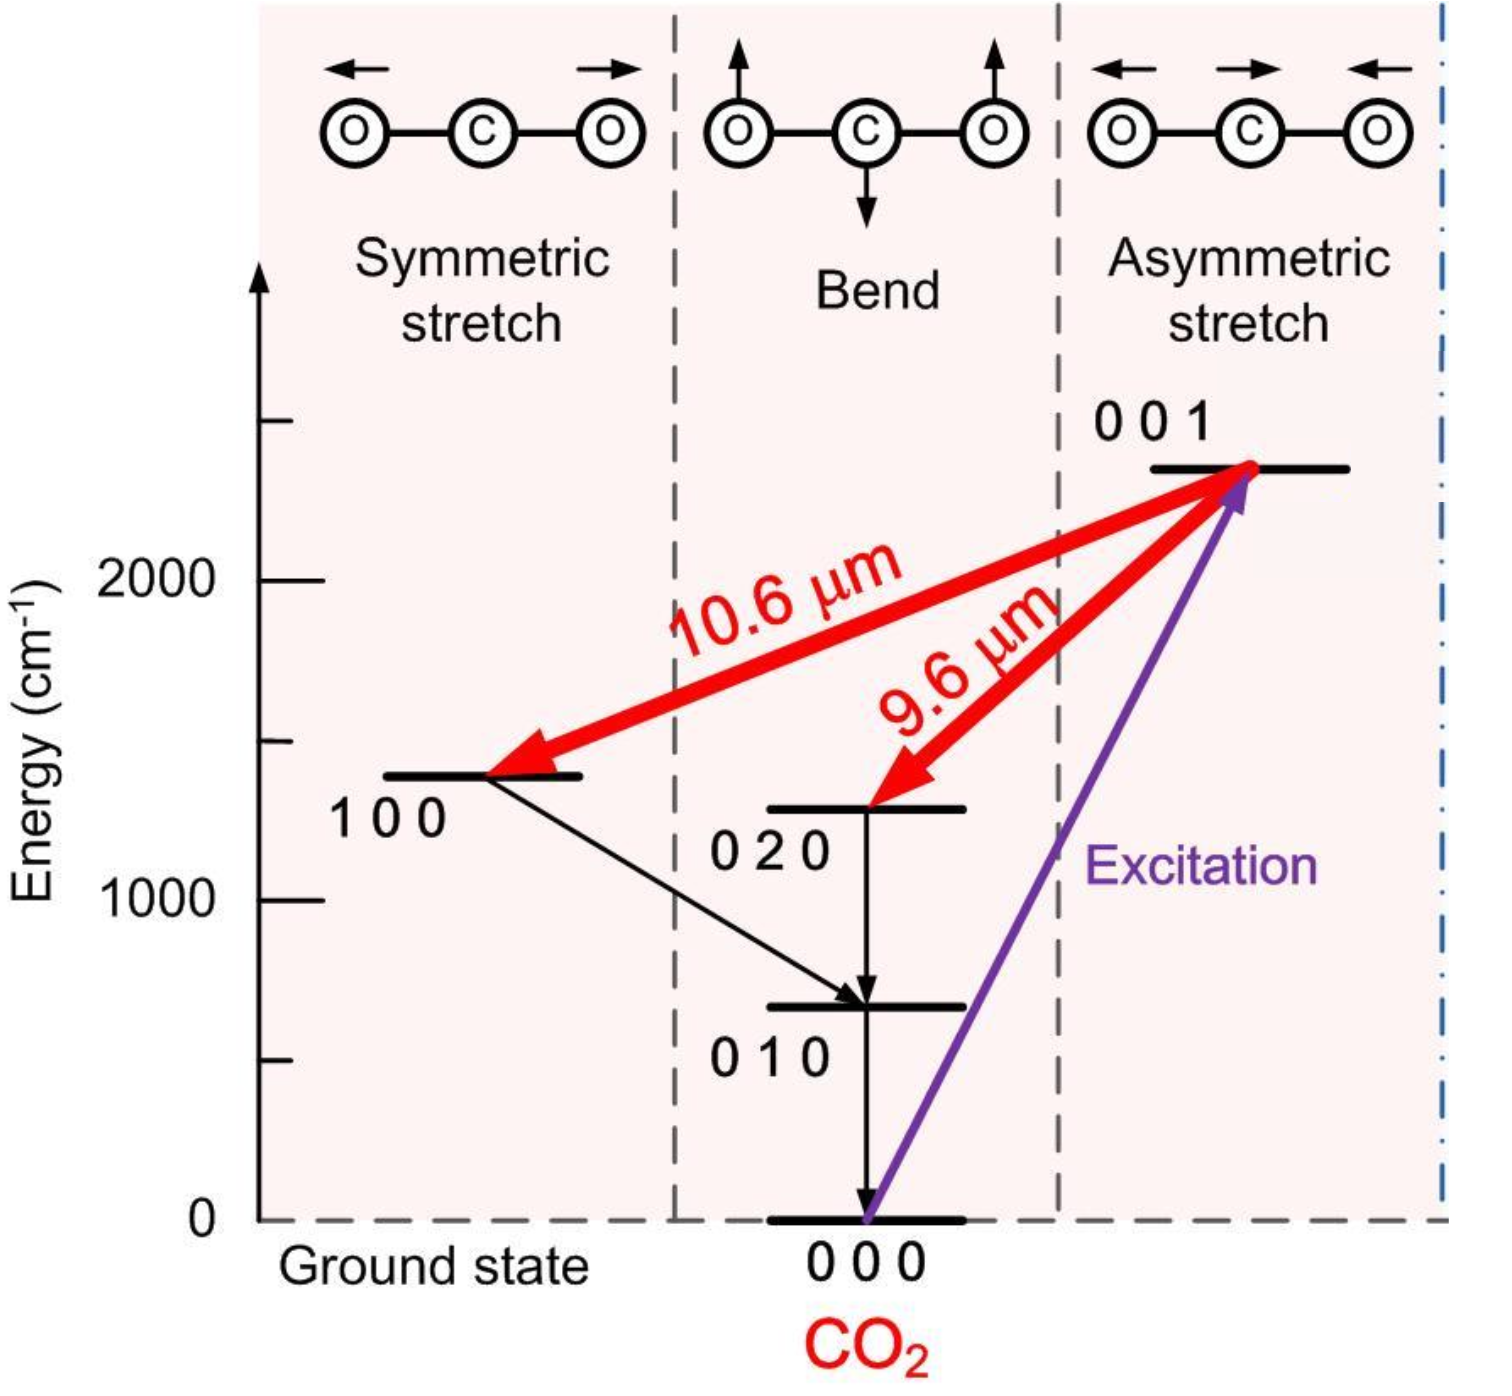
\includegraphics[width=0.35\textwidth]{slike/simpsco2.png}
    \caption{Simplified  energy state of a $CO_2$ molecule. \textit{Source: Lecture Notes.}}
    \label{fig:esco2}
\end{figure}
By adding $N_2$ to the gas mixture, we can pump the $N_2$ and then transfer the energy to the $CO_2$ molecule - figure \ref{fig:n2co2}.
\begin{figure}[h!]
    \centering
    \includegraphics[width=0.35\textwidth]{slike/n2co2.pdf}
    \caption{Pumping with $N_2$. \textit{Source: Lecture Notes.}}
    \label{fig:n2co2}
\end{figure}
We can also add a cooling gas, such as $He$, it is used to transfer heat. Gas mixture ratio for $He:Ne:CO_2$ is $7:2:1$.


\section{Diode Lasers}
Diode lasers are types of lasers that use the bandgap in the semiconductor material, figure \ref{fig:bandsolids}.
The semiconductor material is additionally doped with other elements to determine the properties of the output light - some examples
in table \ref{tab:diodlaser}.

\begin{table}[h!]
    \centering
    \begin{tabular}{|l|l|l|}
    \hline
    \begin{tabular}[c]{@{}l@{}}Laser diode material \\  (active region/substrate)\end{tabular} &
      \begin{tabular}[c]{@{}l@{}}Typical wavelentgth  \\ $\lambda$ {[}nm{]}\end{tabular} &
      Application \\ \hline
    InGaN / GaN, SiC & 380, 405, 450, 470 & data storage                     \\ \hline
    AlGaInP / GaAs   & 635, 650, 670      & laser pointer, DVD player        \\ \hline
    AlGaAs / GaSa &
      720-850 &
      \begin{tabular}[c]{@{}l@{}}CD Player, laser pointers, \\ pumping solid state lasers\end{tabular} \\ \hline
    InGaAs / GaAs    & 900-1100           & Pumping lasers, fiber amplifiers \\ \hline
    InGaP / InP      & 1000-1650          & optical fiber comunications      \\ \hline
    \end{tabular}
    \caption{Diode laser}
    \label{tab:diodlaser}
\end{table}

Light output depends on the current trough the diode, shown on figure \ref{fig:lasdiodchar}. $I_{th}$ is the \textit{threshold current}, at this current the diode starts to emit laser light. 

\begin{figure}[h!]
    \centering
    \includegraphics[width=0.35\textwidth]{slike/diodeIth.pdf}
    \caption{Power/Current characteristics}
    \label{fig:lasdiodchar}
\end{figure}

Figure \ref{fig:lasdiodebeam} shows the beam profile of the laser diode.  Diffraction at crystal-air interface leads to 
strong direction dependant beam-propagation. Intensity profile is \textbf{elliptical}. 
\begin{figure}[h!]
    \centering
    \includegraphics[width=0.35\textwidth]{slike/laserdiode2.pdf}
    \caption{Laser diode beam profile, \textit{Source: Lecture Notes}}
    \label{fig:lasdiodebeam}
\end{figure}

We can achieve very high light output power 
with only one emitter, but the beam quality is very bad. Using diode lasers, we can achieve very high laser power, we can use diode laser bars or stacks of them.
Single emitter can output multiple watts, depending on the width of the resonator. One bar can typically emit from 20 to 100 W, stacks of diodes can emit up to 10 kW.
Shown on figure \ref{fig:diodestacks}.

\begin{figure}[h!]
    \centering
    \includegraphics[width=0.5\textwidth]{slike/diodestack.pdf}
    \caption{Diode, Diode bar, Diode stack \textit{Source: Lecture Notes}}
    \label{fig:diodestacks}
\end{figure}

\subsection{Beam shaping for High-Power diode lasers}
Beam shaping is done using a Fast-Axis collimation using a \textit{high power cylinder lens}.
Each bar has one lens, stacks use additional lenses, as shown on figure \ref{fig:hpc}.
\begin{figure}[h!]
    \centering
    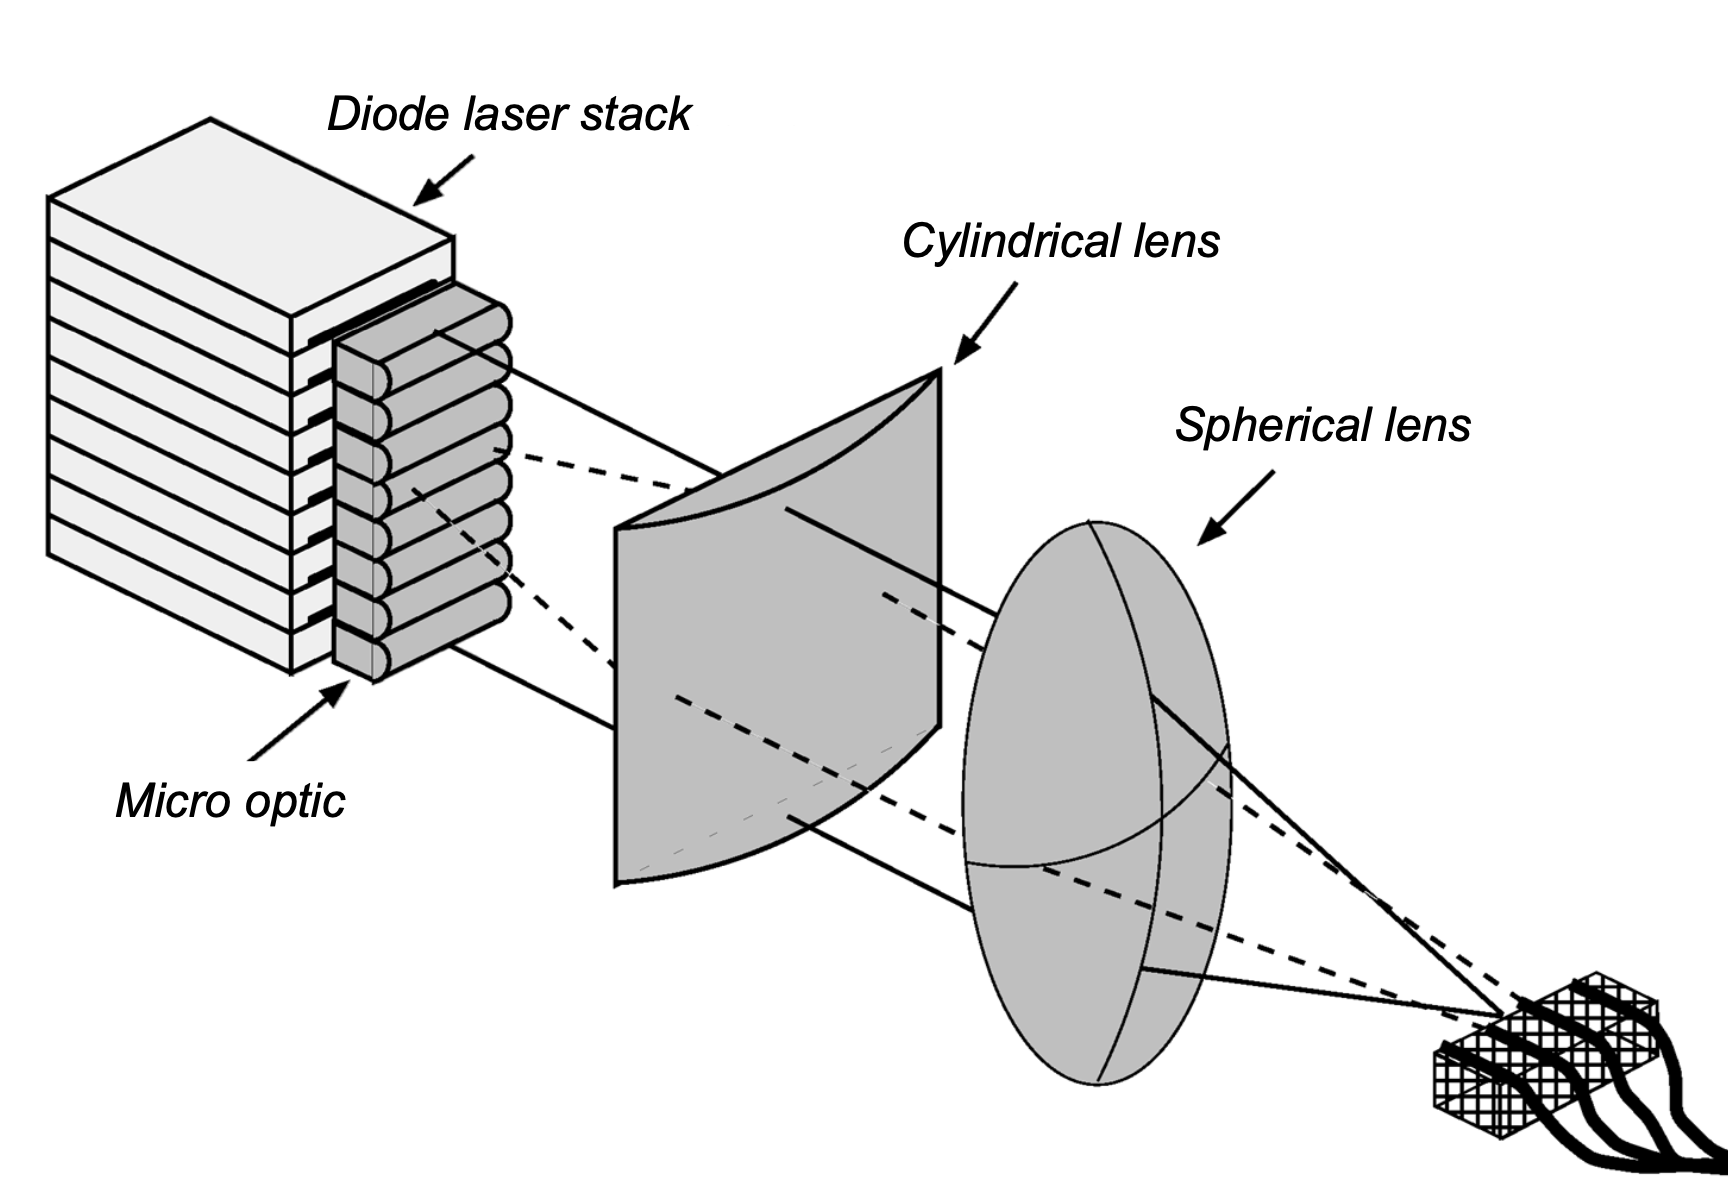
\includegraphics[width=0.5\textwidth]{slike/hpc.png}
    \caption{ High power laser beam focusing. \textit{Source: Lecture Notes}}
    \label{fig:hpc}
\end{figure}

Beam quality of diode lasers is generally \textbf{bad} - not close to Gaussian \pd bad focusing quality.
We \textit{re-image} the beam somewhere else (?).

\subsection{Wavelength and Polarization Multiplexing}

We can increase power of the laser using \textbf{wavelength} and \textbf{polarization} multiplexing.
Laser power increases with consistent $M^2$ - $ P_{total} = L_1 \cdot L_2 \cdot P_0$.
Figures \ref{fig:wm} and \ref{fig:pm} show wavelength and polarization multiplexing.
\begin{figure}[h!]
    \centering
    \includegraphics[width=0.75\textwidth]{slike/wlmp.pdf}
    \caption{Wavelength multiplexing.}
    \label{fig:wm}
\end{figure}
\begin{figure}[h!]
    \centering
    \includegraphics[width=0.25\textwidth]{slike/plmp.pdf}
    \caption{Polarization multiplexing.}
    \label{fig:pm}
\end{figure}

\subsection{High power diode lasers}
Lasers with the power of multiple kilowatts are created by combining stacks. 
If ten stacks with the power of 500 W each are combined, the output power is about 4 kW. 
Losses occur during combination. Spectrum emitted be a high power diode is broad and can change with power, due to thermal variations.
Cooling the diodes is essential, because the temperature effects the BPP/$M^2$.
Figure \ref{fig:tef} shows the temperature effect. 
\begin{figure}[h!]
    \centering
    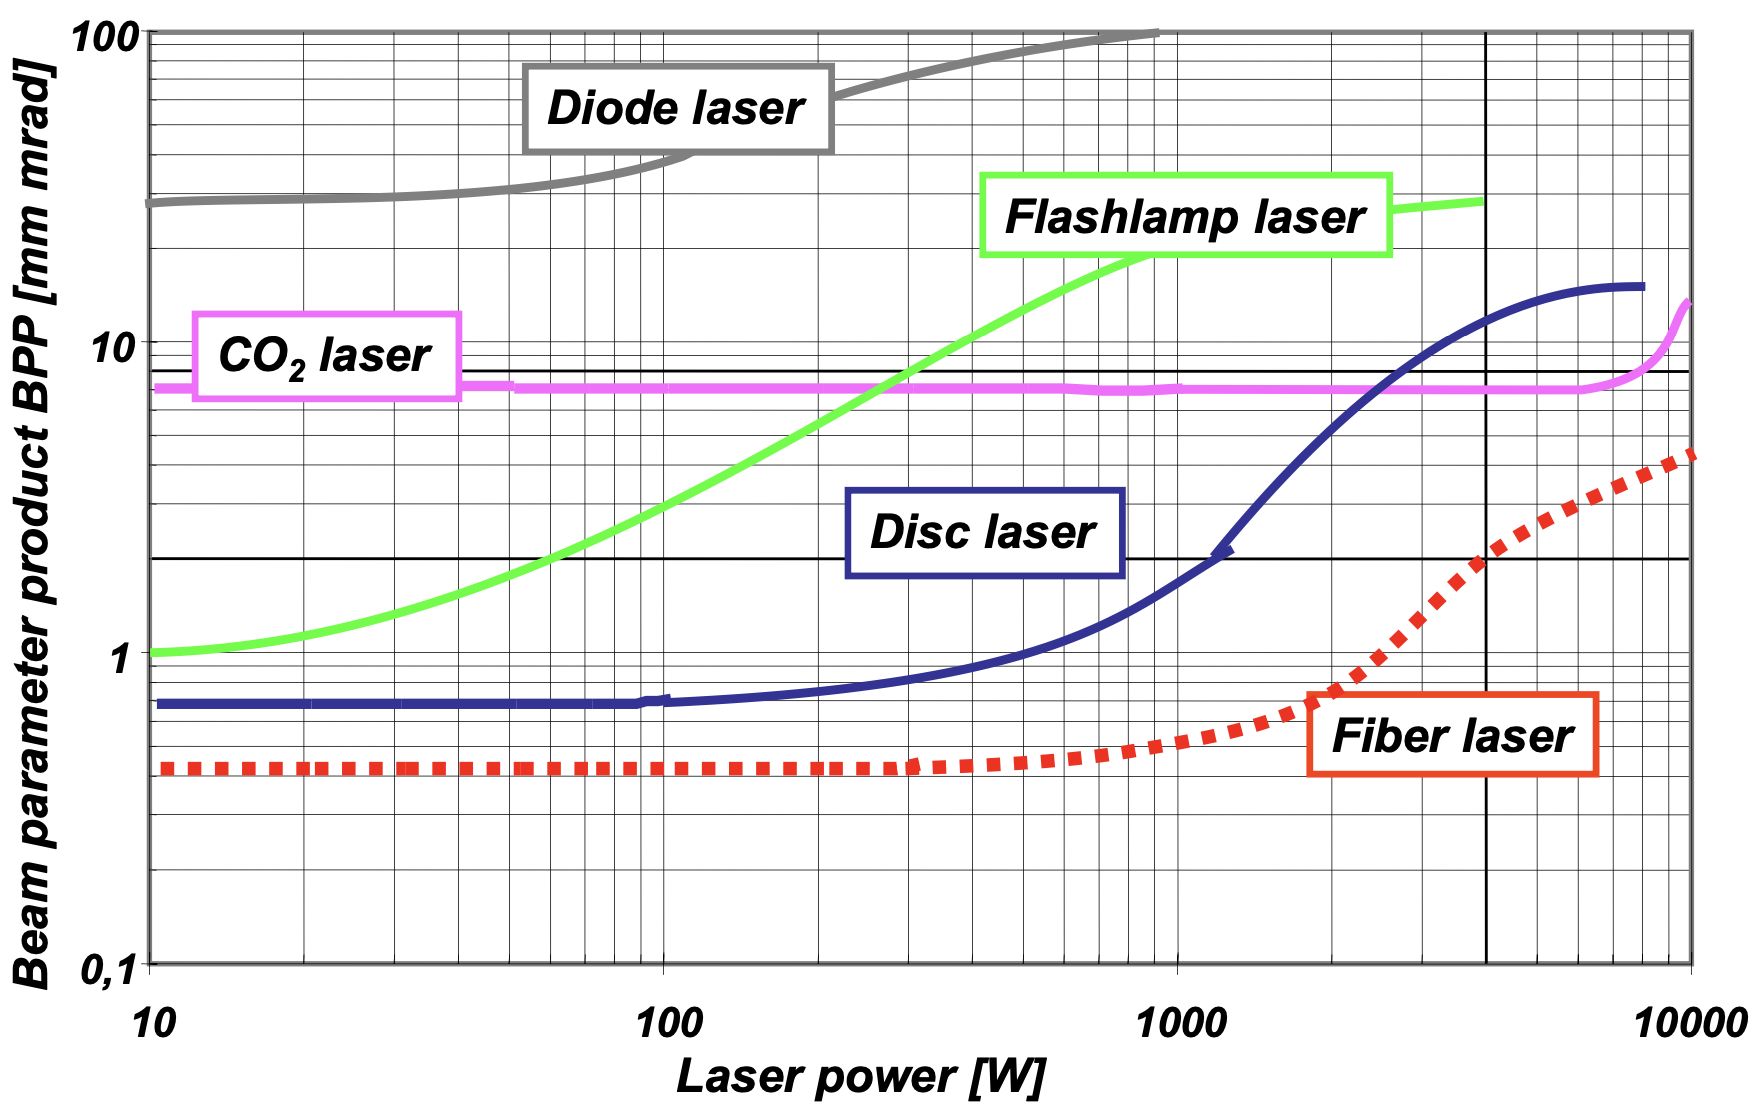
\includegraphics[width=0.5\textwidth]{slike/theffect.png}
    \caption{BPP(T). \textit{Source: Lecture Notes}}
    \label{fig:tef}
\end{figure}

Diode lasers have the highest "wall plug" efficiency. They are cheap to manufacture and operate.

\section{Solid State Lasers}

For some processes, we need both high power and good beam quality. We can use 
\textbf{Solid state lasers}. The active medium in solid state lasers is a doped crystal, such as 
\textit{Nd:YAG, Nd:Glass, Ruby} \dots

Different active media have different optical and physical properties, active medium
is selected based on the desired output parameters. Some popular materials are listed in table \ref{tab:lamssl}
\begin{table}[h!]
    \centering
    \begin{tabular}{|c|c|}
        \hline
        Active medium & Wavelength $\lambda$ \\
        \hline
        Nd:YAG ($Y_3Al_5O_{12}$) & 1064 nm \\
        \hline
        Nd:Glass & 1054 1061, 1064 nm, depends on glass.\\
        \hline
        Nd:YLF ($LiYF_4$) & 1053, 1047 nm \\
        \hline
        Nd:$YVO_4$ & 1064 nm \\
        \hline
    
    \end{tabular}
    \caption{Laser active materials}
    \label{tab:lamssl}
\end{table}

The biggest problem with high power lasers is the management of thermals. 
High temperature leads to \textit{thermal lensing}, which degrades the quality of the beam, and 
losers the pumping efficiency. 

Solid state lasers can be pumped by \textbf{flashlamps} or \textbf{diode lasers}.
Efficiency of source pumping is defined as $\nu = \frac{P_{\lambda}}{P_{in}}$.

\subsection{Flashlamp pumping}

Flashlamp emits a broad spectrum of light, but only one small part of the emitted light will 
pump the active material - this leads to low efficiency of source pumping, between 0.04 and 0.08.


\subsection{Diode laser pumping}
Pumping the laser active material with a diode lasers improves efficiency to 0.3 - 0.5.

\section{Disk Lasers}

Disk lasers are a type of solid state lasers, the active material is a thin disk instead of a long cylinder.
Such a thin disk is easier to cool. Figure \ref{fig:dlaser} shows a simple disk laser.

\begin{figure}[h!]
    \centering
    \includegraphics[width=0.5\textwidth]{slike/disklaser.pdf}
    \caption{Schematics of a disk laser}
    \label{fig:dlaser}
\end{figure}

The thinner the disk, the better we can cool it. The quality of the pump light becomes irrelevant - we can use high power diode lasers.
To improve efficiency, we can let the pump light pass through the disk multiple times - figure 
\ref{fig:dlaser2} shows a real disk laser made by Trumpf. Pump light passes the disk multiple times.
\begin{figure}[h!]
    \centering
    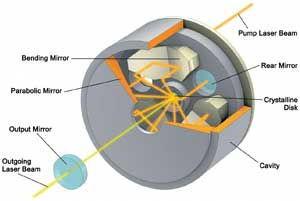
\includegraphics[width=0.35\textwidth]{slike/disklaser2.jpg}
    \caption{Realistic scheme of a disk laser. \sln}
    \label{fig:dlaser2}
\end{figure}

\section{Fiber lasers}
\subsection{Optical fibers}

The main idea of optical fibers is the use of total internal reflection, which is shown on figure 
\ref{fig:totintref}. 
\begin{figure}[h!]
    \centering
    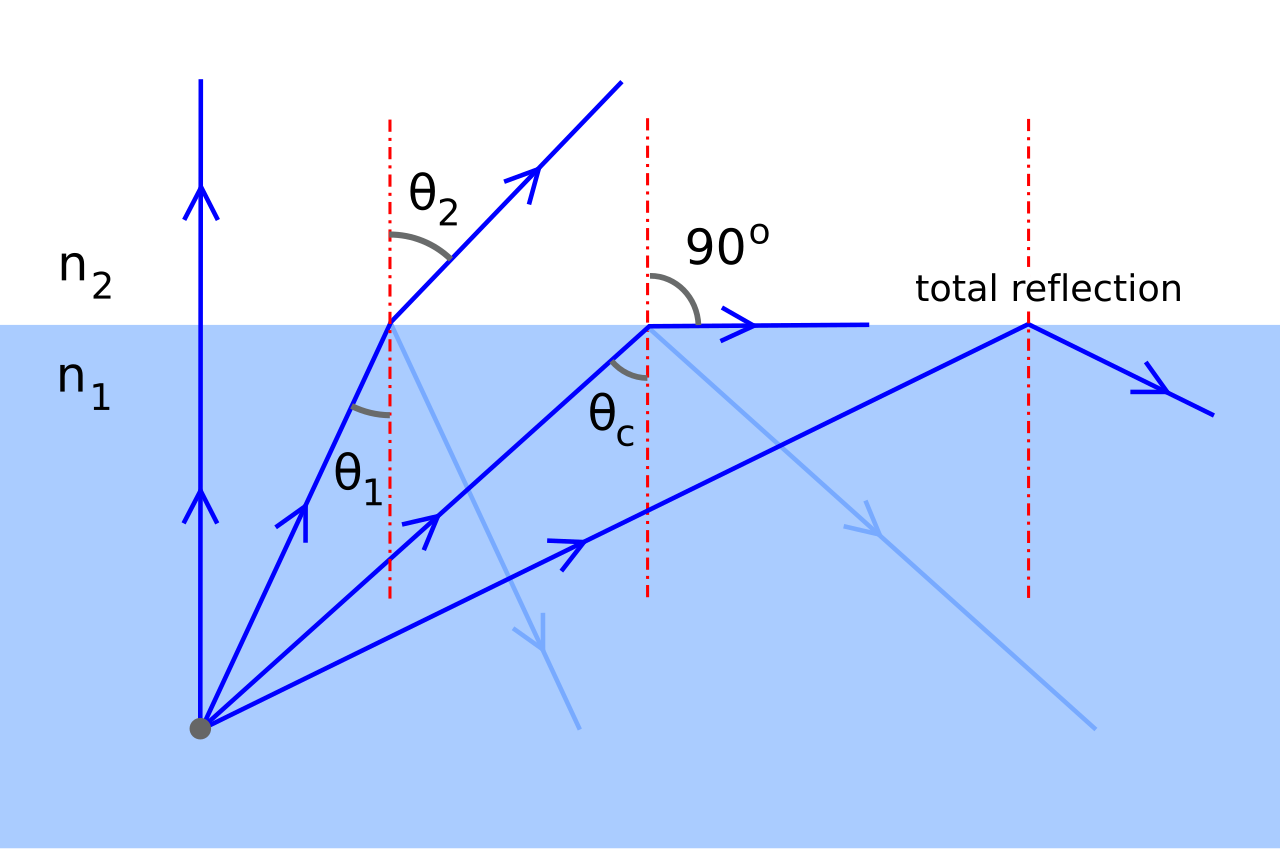
\includegraphics[width=0.5\textwidth]{slike/ReflexionTotal_en.svg.png}
    \caption{Types of reflections}
    \label{fig:totintref}
\end{figure}

Snell's law $n_1 sin \theta_1 = n_2 sin \theta_2$, when $n_2 \le n1 $ and $90° \le \theta_2$ we can derive
$sin\theta_c = \frac{n_2}{n_1} $, where $\theta_C$ is the critical input angle for \textit{total internal reflecton}.

We could use just glass to guide light, but that leads to loss of light when the fiber touches the outside world \pd due to the presence of \textit{evanescent fields} that couple to outside. 

To prevent such losses, we use a core with higher refractive index and use a cladding from a material with lower refractive index to protect the evanescent field. 
Figure \ref{fig:fiber1} shows a cross-section of an optical fiber.  The light is guided in the core.

\begin{figure}[h!]
    \centering
    \includegraphics[width=0.5\textwidth]{slike/optfib.pdf}
    \caption{Cross-section of an optical fiber}
    \label{fig:fiber1}
\end{figure}

Example of a standard optical fiber:


\begin{tabular}{ll}
    Core \pd & Fused silica doped with $GeO_2$ to increase refraction index to $1.470$. \\
    Cladding \pd & Pure fused silica, $n=1.455$.
\end{tabular}


\subsubsection{Coupling beams in to fibers}

Angle at which the light can enter the fiber is determined by the \textbf{Numerical Aperture}, which is calculated by the equation \ref{eq:NA}.
\begin{equation}
    sin(\alpha_g) = \frac{n_2}{n_1}
\end{equation}

\begin{multline}
    NA = n_{Air} sin(\alpha_{max}) = n_1 sin(90° - \alpha_g) = n_1 cos(\alpha_g) =\\
     n_1 \sqrt{1 - sin^2(\alpha_g)} = n_1 \sqrt{1 - (\frac{n_2}{n_1})^2} = \sqrt{n_1^2 - n_2^2}
\label{eq:NA}
\end{multline}

Maximum acceptable input angle is $\alpha_{max}$ is given by the TIR between the core and cladding + refraction at input facet. 
The angle $\alpha_{max}$ constitutes the numerical aperture of a fiber, it is equal to the divergence angle of the light beam at the output. 
Typically, light will have this divergence angle when leaving the fiber. In order to couple two fibers, they have to have matching NA.

\subsubsection{Intensity distribution inside an optical fiber}

Light inside the fiber decomposes into plane waves with different directions.
Core and cladding acts as a circular resonator for plane wave components not parallel
to propagation direction. Shown on figure \ref{fig:opi}.

\begin{figure}[h!]
    \centering
    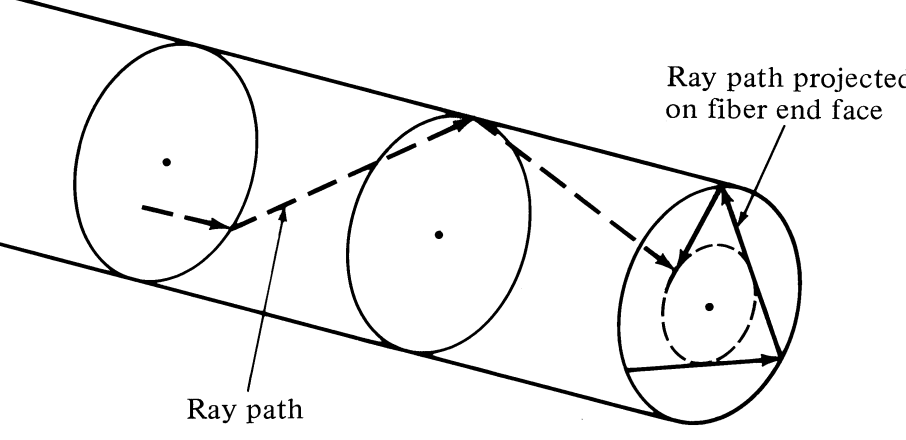
\includegraphics[width=0.5\textwidth]{slike/rof.png}
    \caption{Ray path in optical fiber}
    \label{fig:opi}
\end{figure}


We wish to use \textit{Linearly polarized} modes, which we find by calculating the eigenmodes for the EM-wave equation.

\subsubsection{Single-mode LP fiber}
Ground mode profile is described by the Lorentzian distribution, it deviates from the Gaussian mode by $~1.5\%$. 
Gaussian mode is a good approximation for intensity in single mode fibers.  
Intensity distribution reaches far into the cladding \pd evanescent field of the mode, shown on figure \ref{fig:idfiber}.

\begin{figure}[h!]
    \centering
    \includegraphics[width=0.75\textwidth]{slike/Ifiber.pdf}
    \caption{Single mode fiber distribution}
    \label{fig:idfiber}
\end{figure}

Every single-mode fiber (SMF) has a cut-off frequency (wavelength), at which more LP-modes can propagate, a single mode 
fiber changes into a multi-mode fiber. Rule of thumb is that for single mode operation wavelength has to be larger that the core diameter.

Propagation of ground mode in SMF can be though of  as continuuos focus:
\begin{itemize}
    \item Natural divergence of the beam is compensated by "focusing" action of core and cladding \pd closer to the optical axis of the fiber is 
    higher than outside \pd focussing
    \item Wavefront curvature of ground mode \pd $\infty$, approximately plane wave propagation inside SMF
    \item Description for beam propagation (ABCD method) after out-coupling from SMF given by either by: Mode-field diameter of fiber-NA (beam divergence)
\end{itemize}

\subsubsection{Fiber components necessary for a fiber laser}
\textbf{Filed coupler}

Cores of two fibers are so close together that the evanescent fields overlap into the other core - figure \ref{fig:fcoupler}.  Evanescent filed from 
one core excites the core in another \pd a new co-propagating wave is created. The new evanescent wave will
also propagate its evanescent filed back to the first core.  
The strength of coupling depends on strength of co-propagation filed.
Coupling ratio depends sinusoidally on propagation length between cores. Coupling ratio can be set between 0(?) and 50\%, ratio is determined by
the length of co-propagation and the overlap of evanescent fields - length of fiber distance.
\begin{figure}[h!]
    \centering
    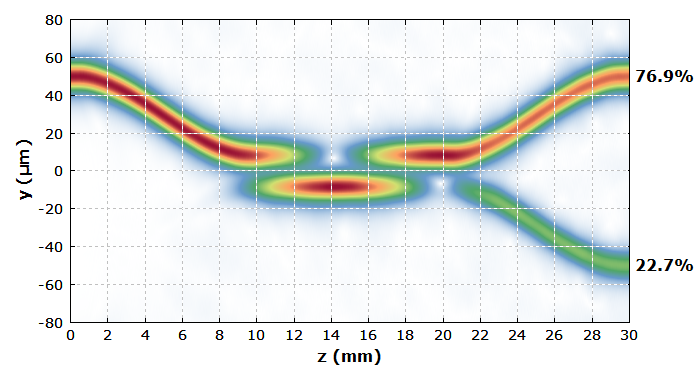
\includegraphics[width=0.5\textwidth]{slike/fcouper.pdf}
    \caption{Evanescent field in the coupler}
    \label{fig:fcoupler}
\end{figure}

\textbf{Fiber Bragg grating}

A fiber bragg grating causes modulation of refractive index inside the core, shown on figure \ref{fig:fbg}.
\begin{figure}[h!]
    \centering
    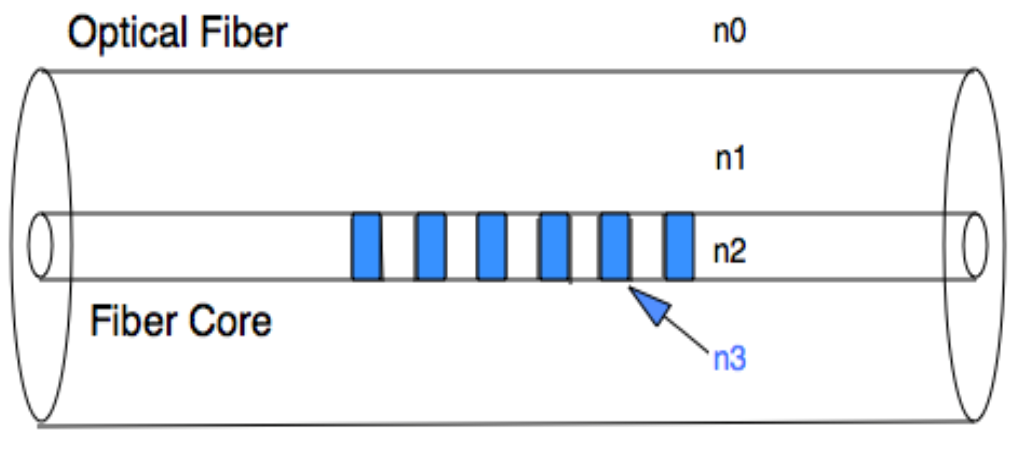
\includegraphics[width=0.35\textwidth]{slike/fbg.png}
    \caption{Fiber Bragg grating}
    \label{fig:fbg}
\end{figure}

Inside the fiber, the waves are reflected from modified zones ($n_3$) and they add up constructively.
During transmission, there is destructive interference from the reflection at modified zones. Bragg grating 
is typically a wavelength selective mirror. The reflectivity and wavelength selectivity is controlled by the number of periods.

\textbf{Wavelength division mulitplexer}

A wavelength division multiplexer combines/splits wavelength from/into different fibers. 
A problem with the coupler is, that the ratio $50:50$, so a combination of a multiplexer and a Fiber Bragg 
grating will lose half of the light.  

\subsection{Fiber laser active media}

Laser active media for a fiber laser is usually made of rare earth elements, 
such as \textit{erbium(ER), neodymium (Nd), ytterbium (Yb)}, in a glass matrix.
Matrix must be glass, otherwise manufacturing is impossible. 
Fiber lasers are solid state, we can only pump them optically. 

\subsection{Fiber laser resonators}
Figure \ref{fig:flr} shows a ring and Bragg-grating based laser resonator.
\begin{figure}[h!]
    \centering
    \includegraphics[width=0.75\textwidth]{slike/flr.pdf}
    \caption{Fiber laser resonator}
    \label{fig:flr}
\end{figure}


Laser resonators are popular due to their compactness and "plug-and-play" capability
of the fibers - they can stay aligned 
for years during industrial use. Heat management is also easier, due 
to the surface area of the cable. They can also achieve good beam quality.

Pumping is done in the entire fiber, shown on figure \ref{fig:ofib}. 
\begin{figure}[h!]
    \centering
    \includegraphics[width=0.35\textwidth]{slike/fopt.pdf}
    \caption{Fiber for pumping}
    \label{fig:ofib}
\end{figure}

Active core and pump lasers are typically separated to homogenize pumping along the entire laser fiber.
The pump wave can be multimode, but must have mode overlap with active core. Laser diode can be used for pumping, the quality ($M^2$) of the pump laser 
is irrelevant to the output quality of the fiber laser. To force the mode overlap with modes from the pump laser, we can
use a non-symmetric pump fiber. 

\subsubsection{Power limiting effects}
Fiber can be damaged due to \textbf{thermals} or \textbf{nonlinear effects}.

In the fiber, there are also \textbf{parasitic effects}:
\begin{itemize}
    \item Thermally induces decrease of pimp efficiency.
    \item Stimulated Brillouin scattering for CW lasers \pd three wave mixing process:
    \begin{itemize}
        \item EM-wave scatters back on sound waves
        \item Back scattered waves interfere with the forward EM-wave \pd standing wavelength
        \item Standing wave is modulated by the Kerr-effect changing the refractive index of the fiber \pd strength of grating increases
        \item EM wave that was travelling in one direction evenly splits into both directions
    \end{itemize}
    \item Amplification of Rayleigh back scattering
    \item Nonlinear effects responsible for wavelength changes
\end{itemize}


To avoid damage caused by nonlinear effects, which reduce laser intensity, we increase the fiber diameter. 
Fiber can then become \textit{multi-modal}, which leads to decrease in beam quality and intensity.
Heat conduction decreases and the laser becomes less efficient.

Fiber lasers have the \textbf{best ratio of surface area to laser beam size}, which leads to high laser power scalability potential 
of all systems. 

High power lasers, such as ytterbium, can reach 100 kW.

\subsubsection{Nd:Glass Laser}
Compared to YAG, glass lasers are highly dopable and easier to produce, however they have \textit{lower} heat conductivity - can only be used 
with low repetition rates. Nd:Glass are used for high power lasers - example: fusion.  
